% !TEX program = xelatex
\documentclass[10pt,a4paper,twocolumn]{article}

% ============================================================================
% ACL / NeurIPS / arXiv Standard Two-Column Conference Geometry & Typography
% Compatible with XeLaTeX (default on Overleaf), LuaLaTeX, and pdfLaTeX
% ============================================================================
\usepackage{iftex}
\ifPDFTeX
  \usepackage[utf8]{inputenc}
  \usepackage[T1]{fontenc}
  \usepackage{lmodern}
\else
  \usepackage{fontspec}
  \usepackage{lmodern}
\fi

\usepackage[a4paper,top=22mm,bottom=22mm,left=19mm,right=19mm,columnsep=6.5mm]{geometry}
\usepackage{microtype}
\usepackage{amsmath,amssymb,amsthm,mathtools}
\usepackage{booktabs}
\usepackage{tabularx}
\usepackage{graphicx}
\usepackage{xcolor}
\usepackage{caption}
\usepackage[round]{natbib}
\usepackage{hyperref}

\definecolor{citeblue}{RGB}{0, 62, 135}

\hypersetup{
  colorlinks=true,
  linkcolor=citeblue,
  citecolor=citeblue,
  urlcolor=citeblue,
  pdftitle={Scaling Laws at the Edge: First-Principles Adaptation, Subspace Allocation, and Quantization Trade-offs for Small Language Models},
  pdfauthor={Sizhe Zhang, Wenyuan Wang, Yuxuan Zhang, Zheyang Dong, Qinqin Zhang}
}

\captionsetup{font=small,labelfont=bf,skip=4pt}
\setlength{\parskip}{0pt}
\setlength{\parindent}{1.1em}
\setlength{\emergencystretch}{1.5em}

\newtheorem{proposition}{Proposition}
\newtheorem{theorem}{Theorem}
\newtheorem{corollary}{Corollary}

% Clean ACL/arXiv Title & Author Block with proper superscripts
\makeatletter
\renewcommand{\maketitle}{%
  \twocolumn[%
    \begin{center}%
      \vspace*{1mm}%
      {\Large\bfseries \@title \par}%
      \vspace{4.5mm}%
      {\normalsize\bfseries
        Sizhe Zhang$^{1}$\hspace{1.4em}%
        Wenyuan Wang$^{1}$\hspace{1.4em}%
        Yuxuan Zhang$^{1}$\hspace{1.4em}%
        Zheyang Dong$^{1}$\hspace{1.4em}%
        Qinqin Zhang$^{1,*}$%
      \par}%
      \vspace{2.2mm}%
      {\small
        $^{1}$School of Mechanical Engineering, Shanghai Jiao Tong University, Shanghai, China\\[2pt]
        $^{*}$Corresponding author: \texttt{zhangqinqin@sjtu.edu.cn}%
      \par}%
      \vspace{5.5mm}%
    \end{center}%
  ]%
}
\makeatother

\title{Scaling Laws at the Edge: First-Principles Adaptation,\\Subspace Allocation, and Quantization Trade-offs for Small Language Models}

\begin{document}

\maketitle

\begin{abstract}
\noindent
Adapting and deploying Small Language Models (SLMs, $26\text{M}$--$1.5\text{B}$ parameters) on memory- and compute-constrained edge accelerators is commonly treated as a scaled-down version of frontier LLM fine-tuning. This scaling assumption is not innocent: in the sub-billion regime, unconstrained full-parameter updates overfit compact domain corpora, attention-only adapters under-parameterize factual recall, and mixed-precision quantization kernels introduce synchronization latencies that outweigh memory-bandwidth savings. We formulate a first-principles framework grounded in the hardware Roofline model, sample-limited intrinsic rank bounds, Transformer subspace specialization, and preference trust-region dynamics. Across a controlled 39-run empirical study spanning four model scales (\texttt{MiniMind2-Small-26M}, \texttt{MiniMind2-104M}, \texttt{Qwen2.5-0.5B}, and \texttt{Qwen2.5-1.5B}) on an NVIDIA Turing (\texttt{sm\_75}) GPU across three zero-leakage diagnostic tasks---multi-hop domain QA (\textsc{CourseQA}), schema-constrained extraction (\textsc{JSONOut}), and out-of-template classification (\textsc{Intent})---we establish four principal results. First, low-rank adaptation acts as an implicit spectral regularizer: on \texttt{MiniMind-26M}, LoRA ($r=16$) improves \textsc{CourseQA} score from $36.80\%$ (8-epoch Full SFT) to $45.71\%$ ($+8.91\%$) while reducing peak training memory by $65.1\%$, and rank ablation on \texttt{Qwen2.5-0.5B} peaks at $r=4$ ($56.88\%$). Second, subspace allocation exhibits a sharp task dichotomy: query-value (\texttt{qv}) adapters saturate syntactic schema extraction ($100.0\%$), whereas factual QA improves monotonically from \texttt{qv} ($18.87\%$) to \texttt{qkvo} ($27.17\%$) and full linear including SwiGLU MLP projections ($32.23\%$). Third, batch-1 decoding on Turing Tensor Cores is governed by dequantization kernel overhead rather than footprint alone: 4-bit NormalFloat (\texttt{NF4}) saves $505.6\text{ MB}$ of static memory while achieving $2.77\times$ higher decoding throughput ($16.01\text{ tok/s}$) than outlier-splitting \texttt{LLM.int8()} ($5.77\text{ tok/s}$). Fourth, Direct Preference Optimization (DPO) on compact models undergoes an acute step-size phase transition, where bounding the learning rate from $5\times 10^{-5}$ to $5\times 10^{-6}$ eliminates off-manifold likelihood displacement and doubles classification accuracy over the zero-shot baseline.
\vspace{1.5mm}
\noindent\textbf{Code Availability:} The complete diagnostic benchmark suites, raw empirical run logs, and adaptation toolkit are open-sourced at: \url{https://github.com/Zhe-SH-CN/edge-slm-scaling-toolkit}.
\end{abstract}

\section{Introduction}

Frontier Large Language Models (LLMs) achieve strong zero-shot generalization across open-domain tasks \citep{brown2020language,achiam2023gpt4}, but their multi-gigabyte memory footprints and high time-to-first-token (TTFT) preclude deployment under strict hardware budgets. In edge workstations, industrial controllers, and single-GPU cloud instances, Small Language Models (SLMs) spanning $10^7$ to $1.5 \times 10^9$ parameters \citep{yang2024qwen25,gong2025minimind} offer a viable alternative when adapted to well-scoped downstream tasks such as technical question answering, schema-constrained JSON telemetry extraction, and deterministic intent routing.

However, directly transferring fine-tuning and post-training quantization recipes from $7\text{B}$--$70\text{B}$ models to the sub-billion regime frequently produces counterintuitive regressions. When operating under tight parameter capacities and first-generation Tensor Core microarchitectures (e.g., NVIDIA Turing \texttt{sm\_75}), four structural tensions emerge:
\begin{itemize}\setlength{\itemsep}{1.5pt}\setlength{\parskip}{0pt}\setlength{\topsep}{3pt}
  \item \textbf{Over-parameterized updates vs.\ sample complexity.} Because a $26\text{M}$-parameter model fits in $<500\text{ MB}$ of training VRAM, full-parameter supervised fine-tuning (Full SFT) is computationally inexpensive. Yet when the downstream corpus contains $N \sim 10^2$ domain examples, unconstrained rank-$d_{\text{model}}$ gradient updates memorize surface phrasing in trailing singular directions rather than isolating the low-dimensional task signal \citep{aghajanyan2021intrinsic,hu2022lora}.
  \item \textbf{Syntactic routing vs.\ factual memory subspaces.} Standard parameter-efficient fine-tuning (PEFT) conventions attach low-rank adapters only to attention query and value projections (\texttt{qv}) \citep{hu2022lora}. While sufficient for re-routing surface syntax, this leaves feed-forward network (FFN) key-value memories \citep{geva2021transformer,meng2022locating} frozen during domain knowledge injection.
  \item \textbf{Memory bandwidth vs.\ dequantization kernel overhead.} Weight-only quantization (\texttt{INT8}, \texttt{NF4}) reduces static VRAM \citep{dettmers2022llm,dettmers2023qlora}. At batch size $B=1$, however, the wall-clock time saved by transferring fewer bytes across memory bus $B_{\text{mem}}$ on a $0.5\text{B}$ model is only $1$--$2\text{ ms/token}$ \citep{williams2009roofline}; any dynamic activation-thresholding or host-device synchronization overhead directly inflates decoding latency.
  \item \textbf{Off-manifold likelihood displacement in preference alignment.} Direct Preference Optimization (DPO) \citep{rafailov2023direct} eliminates the explicit reward model by contrasting chosen and rejected completions directly in policy log-space. On compact models with shared prompt prefixes, aggressive negative gradients rapidly drain probability mass from valid label tokens toward out-of-vocabulary strings \citep{pal2024smaug,tajwar2024preference}.
\end{itemize}

\begin{figure*}[t]
  \centering
  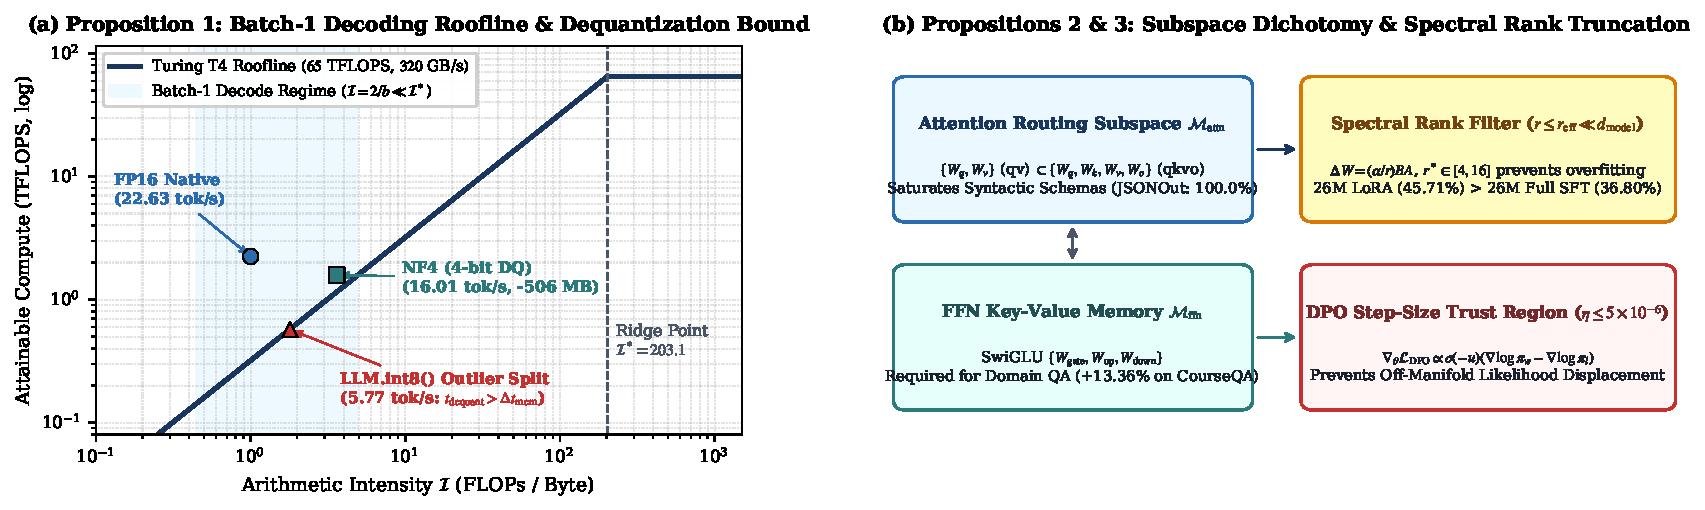
\includegraphics[width=\textwidth]{fig1_framework.pdf}
  \caption{\textbf{First-principles adaptation and deployment framework for edge SLMs.} \textbf{(a)} Hardware Roofline model for NVIDIA Turing \texttt{sm\_75} ($65\text{ TFLOPS}$, $320\text{ GB/s}$). Batch-1 decoding operates in the memory-bound regime ($\mathcal{I} \ll \mathcal{I}^*$), where \texttt{LLM.int8()} outlier decomposition incurs synchronization overhead exceeding bandwidth savings (Proposition~\ref{prop:quant}). \textbf{(b)} Structural decomposition of Transformer adaptation into attention routing ($\mathcal{M}_{\text{attn}}$), FFN key-value memory ($\mathcal{M}_{\text{ffn}}$), spectral rank truncation ($r \le r_{\text{eff}}$), and DPO trust-region step control.}
  \label{fig:framework}
\end{figure*}

\paragraph{Problem statement and system model.}
Given a pre-trained causal Transformer $\pi_{\theta_0}$ with parameter count $\Phi \in [2.6\times 10^7, 1.54\times 10^9]$, a target task distribution $\mathcal{D}$ with $N$ labeled training examples, and a hardware accelerator characterized by peak compute $C_{\text{peak}}$, memory bandwidth $B_{\text{mem}}$, and physical memory ceiling $M_{\max}$, we seek an adaptation operator $\theta_0 \mapsto \theta = \theta_0 + \Delta\theta$ and an inference quantization bit-width $b \in \{4, 8, 16\}$ that maximize out-of-sample task performance $\mathcal{P}(\pi_\theta)$ subject to $M_{\text{peak}}(\Phi, b) \le M_{\max}$ and per-token latency constraints. Figure~\ref{fig:framework} summarizes our analytical framework.

\paragraph{Contributions.}
\begin{itemize}\setlength{\itemsep}{1.5pt}\setlength{\parskip}{0pt}\setlength{\topsep}{3pt}
  \item \textbf{First-principles latency and rank bounds for SLMs.} We derive the exact dequantization latency inequality under the Roofline model (Proposition~\ref{prop:quant}) and the sample-limited numerical rank bound for assistant-masked updates (Proposition~\ref{prop:rank}), explaining why low-rank constraints act as a spectral regularizer in compact regimes (§\ref{sec:theory}).
  \item \textbf{Task-dependent subspace hierarchy.} We formalize and empirically verify a functional dichotomy between attention routing ($\mathcal{M}_{\text{attn}}$) and FFN key-value storage ($\mathcal{M}_{\text{ffn}}$): \texttt{qv} adapters saturate strict JSON schema extraction ($100.0\%$), whereas domain QA requires adapting FFN projections for a $+13.36\%$ gain over \texttt{qv} (§\ref{sec:subspace_theory}, §\ref{sec:exp_ablation}).
  \item \textbf{Controlled 39-run scaling, quantization, and alignment audit.} Across four model scales ($26\text{M}$ to $1.5\text{B}$) and three zero-leakage diagnostic tasks, we map the latency--memory Pareto frontier of \texttt{FP16}, \texttt{LLM.int8()}, and \texttt{NF4}, and identify the exact step-size phase transition ($\eta = 5\times 10^{-5} \to 5\times 10^{-6}$) that prevents likelihood displacement in compact DPO (§\ref{sec:experiments}).
\end{itemize}

\section{First-Principles Theoretical Framework}
\label{sec:theory}

\subsection{Hardware Roofline and Memory State Decomposition}
\label{sec:roofline}

Let $\Phi$ denote the total parameter count of a causal Transformer deployed on an accelerator with peak half-precision compute $C_{\text{peak}}$ and memory bandwidth $B_{\text{mem}}$. On an NVIDIA Tesla T4 (\texttt{sm\_75}, 40 SMs, $14.56\text{ GiB}$ GDDR6), $C_{\text{peak}}^{\text{FP16}} = 65\text{ TFLOPS}$ and $B_{\text{mem}} = 320\text{ GB/s}$, placing the Roofline ridge point at $\mathcal{I}^* = C_{\text{peak}} / B_{\text{mem}} = 203.1\text{ FLOPs/byte}$ \citep{williams2009roofline}. Because Turing Tensor Cores lack native hardware \texttt{bfloat16} pipelines and Ampere-only \texttt{sm\_80+} instructions required by FlashAttention-2 \citep{dao2023flashattention2}, hardware-optimal execution requires \texttt{float16} weights paired with memory-efficient Scaled Dot-Product Attention (SDPA) \citep{rabe2021self}.

\paragraph{Training memory decomposition.}
Full-parameter mixed-precision SFT with AdamW \citep{loshchilov2019decoupled} requires storing \texttt{FP16} parameters ($2\Phi$ bytes), \texttt{FP16} gradients ($2\Phi$ bytes), and \texttt{FP32} master weights plus first and second moments ($m_t, v_t$, totaling $12\Phi$ bytes):
\begin{equation}
  M_{\text{train}}^{\text{Full}}(\Phi) = 16\Phi + M_{\text{act}}(B, L, d_{\text{model}}).
  \label{eq:mem_full}
\end{equation}
For $\Phi = 2.6 \times 10^7$ (\texttt{MiniMind-26M}), $16\Phi \approx 416\text{ MB}$, enabling full-parameter training in $<0.5\text{ GB}$ VRAM. Conversely, for $\Phi = 1.54 \times 10^9$ (\texttt{Qwen2.5-1.5B}), $16\Phi \approx 24.6\text{ GB}$, exceeding the $14.56\text{ GiB}$ physical limit prior to activation allocation. Freezing the base model in 4-bit NormalFloat with double quantization ($b \approx 0.55\text{ bytes/param}$) and updating only low-rank adapters $\Phi_{\text{LoRA}} \ll \Phi$ \citep{dettmers2023qlora} reduces training state memory to:
\begin{equation}
  M_{\text{train}}^{\text{QLoRA}}(\Phi) = 0.55\Phi + 16\Phi_{\text{LoRA}} + M_{\text{act}}^{\text{ckpt}},
  \label{eq:mem_qlora}
\end{equation}
bounding the static and optimizer state footprint of a $1.54\text{B}$ model below $1.2\text{ GB}$.

\begin{proposition}[Quantized Decoding Latency Condition]
\label{prop:quant}
During batch-1 autoregressive decoding ($B=1$), generating each token requires $2\Phi$ FLOPs and streams $b\Phi$ bytes of model weights from global memory, resulting in arithmetic intensity $\mathcal{I}_{\text{decode}} = 2/b \ll \mathcal{I}^*$. Let $t_{\text{dequant}}(b)$ denote the per-token kernel execution and synchronization overhead of dequantizing $b$-bit weights to \texttt{FP16}. Weight quantization from $b_0=2$ (\texttt{FP16}) to $b < 2$ reduces per-token decoding latency $t_{\text{token}}(b)$ if and only if:
\begin{equation}
  t_{\text{dequant}}(b) < \Delta t_{\text{mem}}(b) \triangleq \frac{(2 - b)\Phi}{B_{\text{mem}}}.
  \label{eq:dequant_bound}
\end{equation}
\end{proposition}
\noindent\textit{Derivation.} Under the memory-bound regime of the Roofline model ($\mathcal{I}_{\text{decode}} \le 4 \ll 203.1$), ideal memory-transfer time is $b\Phi / B_{\text{mem}}$. Adding dequantization kernel time $t_{\text{dequant}}(b)$ yields $t_{\text{token}}(b) \approx b\Phi / B_{\text{mem}} + t_{\text{dequant}}(b) + t_{\text{compute}}$. Comparing $t_{\text{token}}(b) < t_{\text{token}}(2)$ with $t_{\text{dequant}}(2) = 0$ immediately yields Inequality~(\ref{eq:dequant_bound}). $\square$

For a sub-billion model ($\Phi = 4.94 \times 10^8$, \texttt{Qwen2.5-0.5B}) on T4 ($B_{\text{mem}} = 320\text{ GB/s}$), reducing weight precision from \texttt{FP16} ($b=2$) to \texttt{INT8} ($b \approx 1.1$) or \texttt{NF4} ($b \approx 0.55$) yields a theoretical memory-transfer reduction $\Delta t_{\text{mem}}$ of only $1.39\text{ ms}$ to $2.24\text{ ms}$ per token. Any quantization scheme that incurs dynamic per-layer outlier extraction and host-device stream synchronization (\texttt{LLM.int8()}; \citealp{dettmers2022llm}) with $t_{\text{dequant}} \gg 2.2\text{ ms}$ will strictly slow down inference despite reducing VRAM.

\subsection{Intrinsic Rank Bound and Spectral Regularization}
\label{sec:rank_theory}

For a pre-trained projection $W_0 \in \mathbb{R}^{d_{\text{out}} \times d_{\text{in}}}$, LoRA \citep{hu2022lora} constrains the parameter update to $\Delta W = (\alpha / r) B A$, where $B \in \mathbb{R}^{d_{\text{out}} \times r}$, $A \in \mathbb{R}^{r \times d_{\text{in}}}$, and $r \ll \min(d_{\text{in}}, d_{\text{out}})$.

\begin{proposition}[Sample-Limited Rank Upper Bound]
\label{prop:rank}
Consider assistant-masked cross-entropy training over $N$ examples with average target completion length $\bar{L}_{\text{ans}}$ tokens. At each layer, the cumulative first-order gradient update $\Delta W_{\text{SFT}} = -\eta \sum_{i=1}^{N} \sum_{t=1}^{\bar{L}_{\text{ans}}} g_{i,t} h_{i,t}^\top$ is a linear combination of at most $N \bar{L}_{\text{ans}}$ rank-1 outer products between backpropagated output gradients $g_{i,t} \in \mathbb{R}^{d_{\text{out}}}$ and input activations $h_{i,t} \in \mathbb{R}^{d_{\text{in}}}$. Its numerical rank at singular-value threshold $\epsilon > 0$ satisfies:
\begin{equation}
  r_{\text{eff}}(\Delta W_{\text{SFT}}, \epsilon) \le \min\!\big(d_{\text{in}},\, d_{\text{out}},\, \kappa(\epsilon) N \bar{L}_{\text{ans}}\big),
  \label{eq:rank_bound}
\end{equation}
where $\kappa(\epsilon) \in (0, 1]$ is the fraction of linearly independent token-level gradient directions exceeding $\epsilon$.
\end{proposition}
When adapting an SLM on a compact domain dataset ($N \approx 10^2$, $\bar{L}_{\text{ans}} \approx 25$), strong syntactic and semantic correlation across examples concentrates the task-relevant gradient energy into the top $r^* \in [4, 16]$ singular vectors ($\kappa(\epsilon) \ll 0.01$). Unconstrained Full SFT updates all $\min(d_{\text{in}}, d_{\text{out}}) \ge 512$ singular directions, allowing trailing singular vectors to memorize idiosyncratic lexical artifacts of the training split. Enforcing $\text{rank}(\Delta W) \le r$ acts as a hard spectral truncation filter that projects updates onto the principal task subspace while leaving the orthogonal complement $\ker(A)$ invariant.

\subsection{Subspace Specialization: Attention vs.\ FFN}
\label{sec:subspace_theory}

Each Transformer layer contains attention projections $\mathcal{M}_{\text{attn}} = \{W_q, W_k, W_v, W_o\}$ and gated MLP/FFN projections $\mathcal{M}_{\text{ffn}} = \{W_{\text{gate}}, W_{\text{up}}, W_{\text{down}}\}$. Mechanistic interpretability studies \citep{geva2021transformer,meng2022locating} show that FFN layers act as key-value memories where $W_{\text{gate}}, W_{\text{up}}$ detect input patterns and $W_{\text{down}}$ projects factual value vectors into the residual stream, whereas attention heads route contextual tokens and govern output syntax. This structural division implies two distinct adaptation regimes:
\begin{enumerate}\setlength{\itemsep}{1pt}\setlength{\parskip}{0pt}\setlength{\topsep}{2pt}
  \item \textbf{Syntax-constrained extraction (\textsc{JSONOut}, \textsc{Intent}).} All entity values are explicitly supplied in the prompt context; adaptation only needs to suppress conversational preamble and enforce output schema grammar. Adapting $\mathcal{M}_{\text{qv}} = \{W_q, W_v\}$ suffices to saturate test accuracy: $\mathcal{P}(\mathcal{M}_{\text{qv}}) \approx \mathcal{P}(\mathcal{M}_{\text{attn}} \cup \mathcal{M}_{\text{ffn}})$.
  \item \textbf{Knowledge-intensive QA (\textsc{CourseQA}).} Answering multi-hop technical questions without external context requires modifying factual associations stored in FFN weights, inducing a strict monotonic ordering:
  \begin{equation}
    \mathcal{P}(\mathcal{M}_{\text{qv}}) < \mathcal{P}(\mathcal{M}_{\text{attn}}) < \mathcal{P}(\mathcal{M}_{\text{attn}} \cup \mathcal{M}_{\text{ffn}}).
    \label{eq:subspace_ineq}
  \end{equation}
\end{enumerate}

\subsection{Likelihood Displacement in Compact DPO}
\label{sec:dpo_theory}

Given preference triples $(x, y_w, y_l)$, DPO \citep{rafailov2023direct} optimizes:
\begin{equation}
\begin{aligned}
  \mathcal{L}_{\text{DPO}}(\theta) = -\mathbb{E}\bigg[\log \sigma\Big(&\beta \log \frac{\pi_\theta(y_w|x)}{\pi_{\text{ref}}(y_w|x)} \\
  &- \beta \log \frac{\pi_\theta(y_l|x)}{\pi_{\text{ref}}(y_l|x)}\Big)\bigg].
\end{aligned}
\label{eq:dpo_loss}
\end{equation}
Let $u(x, y_w, y_l) = \beta \log \frac{\pi_\theta(y_w|x)}{\pi_{\text{ref}}(y_w|x)} - \beta \log \frac{\pi_\theta(y_l|x)}{\pi_{\text{ref}}(y_l|x)}$. The gradient with respect to $\theta$ is:
\begin{equation}
\begin{aligned}
  \nabla_\theta \mathcal{L}_{\text{DPO}} = -\beta\,\mathbb{E}\Big[\sigma(-u)\big(&\nabla_\theta \log \pi_\theta(y_w|x) \\
  &- \nabla_\theta \log \pi_\theta(y_l|x)\big)\Big].
\end{aligned}
\label{eq:dpo_grad}
\end{equation}
In discrete classification (\textsc{Intent}), $y_w$ and $y_l$ are short snake\_case label tokens conditioned on an identical prompt $x$, so their hidden-state representations $\nabla_\theta \log \pi_\theta(y_w|x)$ and $\nabla_\theta \log \pi_\theta(y_l|x)$ exhibit high cosine similarity in the final projection layer. When the learning rate $\eta$ exceeds the local trust region ($\eta = 5\times 10^{-5}$), the repulsive gradient $-\nabla_\theta \log \pi_\theta(y_l|x)$ destabilizes shared token embeddings, shifting probability mass away from the entire valid label set $\mathcal{Y}$ toward arbitrary out-of-vocabulary tokens (likelihood displacement; \citealp{pal2024smaug,tajwar2024preference}). Preventing collapse without an explicit SFT stage requires constraining $\eta \le 5\times 10^{-6}$.

\begin{table}[t]
\centering
\resizebox{\columnwidth}{!}{%
\begin{tabular}{llrrrr}
\toprule
\textbf{Dataset} & \textbf{Task Regime} & \textbf{Train} & \textbf{Dev} & \textbf{Test} & \textbf{Total} \\
\midrule
\textsc{CourseQA} & Multi-hop domain QA (8 topics) & 104 & 34 & 32 & 170 \\
\textsc{JSONOut} & Schema extraction (4 schemas) & 384 & 128 & 128 & 640 \\
\textsc{Intent} & Out-of-template routing (6 classes) & 576 & 192 & 192 & 960 \\
\midrule
\textbf{Total} & \textbf{Zero-leakage benchmark} & \textbf{1,064} & \textbf{354} & \textbf{352} & \textbf{1,770} \\
\bottomrule
\end{tabular}%
}
\caption{\textbf{Diagnostic benchmark statistics.} Cross-split ID overlap is strictly $\emptyset$ across all tasks; \textsc{Intent} test queries use held-out syntactic templates disjoint from train and dev.}
\label{tab:dataset}
\end{table}

\section{Experimental Setup}
\label{sec:experiments}

We organize our empirical evaluation around four falsifiable questions corresponding to Section~\ref{sec:theory}: \textbf{Q1 (Spectral regularization)}: Does rank-restricted LoRA outperform unconstrained Full SFT on compact QA corpora, and how does optimal rank scale? \textbf{Q2 (Subspace dichotomy)}: When do attention-only (\texttt{qv}) adapters suffice, and when must FFN projections (\texttt{all-linear}) be unlocked? \textbf{Q3 (Quantized decoding Roofline)}: Does empirical batch-1 throughput on Turing Tensor Cores obey Proposition~\ref{prop:quant} across \texttt{FP16}, \texttt{LLM.int8()}, and \texttt{NF4}? \textbf{Q4 (DPO trust-region stability)}: How does learning-rate scaling govern likelihood displacement vs.\ boundary alignment in compact DPO?

\subsection{Zero-Leakage Diagnostic Benchmark}

To rule out pre-training memorization and evaluate genuine task adaptation, we construct a 1,770-sample benchmark (Table~\ref{tab:dataset}) with deterministic seed $42$ and programmatic verification that train/dev/test ID intersections are strictly empty:
\begin{itemize}\setlength{\itemsep}{1pt}\setlength{\parskip}{0pt}\setlength{\topsep}{2pt}
  \item \textbf{\textsc{CourseQA} ($N=170$).} Technical question-answer pairs stratified across eight computer science domains (data structures, asymptotic complexity, operating systems, computer networks, relational databases, boolean logic, sorting, and graph algorithms). Each item is evaluated via normalized Exact Match (EM), character-level Token-F1, and answer containment (\text{Contains}). To reflect question structure accurately, each item carries a primary scorer tag $\text{scorer}(i) \in \{\text{EM}, \text{F1}\}$ (EM for short factoid/complexity items; Token-F1 for multi-clause definitional items), and the headline \text{Overall} score is the exact per-sample average $\frac{1}{|D_{\text{test}}|}\sum_{i} s_{\text{scorer}(i)}(\hat{y}_i, y_i)$.
  \item \textbf{\textsc{JSONOut} ($N=640$).} Unstructured natural language descriptions mapped to four strict JSON schemas (\texttt{course\_info}, \texttt{student\_grade}, \texttt{lab\_schedule}, \texttt{bug\_report}) requiring semantic-to-boolean type conversion (e.g., mapping ``pending fix'' to \texttt{resolved: false}). We report \text{JSON Parse Rate} (\texttt{json.loads} success), strict \text{Schema Valid Rate} (exact key set and Python types, used as \text{Overall}), and key-level \text{Field Accuracy}.
  \item \textbf{\textsc{Intent} ($N=960$).} Utterances balanced across six routing classes (\texttt{deadline\_extension}, \texttt{grade\_appeal}, \texttt{concept\_question}, \texttt{debug\_help}, \texttt{env\_setup}, \texttt{team\_matching}). While train and dev splits are generated from declarative templates, the 192 test queries use disjoint interrogative and colloquial templates. We report \text{Accuracy} (\text{Overall}), \text{Macro-F1}, and out-of-vocabulary \text{Unmapped Rate}.
\end{itemize}

\begin{table*}[t]
\centering
\resizebox{\textwidth}{!}{%
\begin{tabular}{lllcrrrrrr}
\toprule
\textbf{Model Scale} & \textbf{Task} & \textbf{Method} & \textbf{Schedule / Rank} & \textbf{Primary Metric 1} & \textbf{Primary Metric 2} & \textbf{Overall} & \textbf{Gain ($\Delta$)} & \textbf{Time (s)} & \textbf{Peak VRAM (MB)} \\
\midrule
\multicolumn{10}{l}{\textit{Tier 1: Ultra-Compact Models (\texttt{MiniMind2-Small}, $\Phi = 26\text{M}$ \& \texttt{MiniMind2}, $\Phi = 104\text{M}$)}} \\
\texttt{MiniMind-26M} & \textsc{CourseQA} & Zero-Shot & --- & EM: 0.0000 & F1: 0.1260 & 0.1025 & --- & 80.03 & 60.0 \\
\texttt{MiniMind-26M} & \textsc{CourseQA} & Full SFT & 3 ep / Full & EM: 0.0625 & F1: 0.2123 & 0.1870 & $+0.0845$ & 4.37 & 473.7 \\
\texttt{MiniMind-26M} & \textsc{CourseQA} & Full SFT & 8 ep / Full & EM: 0.2812 & F1: 0.4055 & 0.3680 & $+0.2655$ & 5.57 & 375.0 \\
\texttt{MiniMind-26M} & \textsc{CourseQA} & \textbf{LoRA} & 8 ep / $r=16$ & \textbf{EM: 0.4062} & \textbf{F1: 0.5370} & \textbf{0.4571} & $\mathbf{+0.3546}$ & 16.22 & \textbf{130.9} \\
\texttt{MiniMind-104M} & \textsc{CourseQA} & Zero-Shot & --- & EM: 0.0000 & F1: 0.1458 & 0.1034 & --- & 29.09 & 531.7 \\
\texttt{MiniMind-104M} & \textsc{CourseQA} & Full SFT & 8 ep / Full & EM: 0.3438 & F1: 0.4663 & 0.4256 & $+0.3222$ & 14.00 & 1431.5 \\
\texttt{MiniMind-26M} & \textsc{JSONOut} & Zero-Shot & --- & Parse: 0.0391 & Field: 0.0016 & 0.0000 & --- & 253.32 & 133.1 \\
\texttt{MiniMind-26M} & \textsc{JSONOut} & \textbf{Full SFT} & 4 ep / Full & \textbf{Parse: 1.0000} & \textbf{Field: 1.0000} & \textbf{1.0000} & $\mathbf{+1.0000}$ & 105.13 & 372.1 \\
\texttt{MiniMind-26M} & \textsc{Intent} & Zero-Shot & --- & Acc: 0.0000 & F1: 0.0000 & 0.0000 & --- & 46.00 & 370.9 \\
\texttt{MiniMind-26M} & \textsc{Intent} & \textbf{Full SFT} & 4 ep / Full & \textbf{Acc: 1.0000} & \textbf{F1: 1.0000} & \textbf{1.0000} & $\mathbf{+1.0000}$ & 11.80 & 376.0 \\
\midrule
\multicolumn{10}{l}{\textit{Tier 2: Sub-Billion \& Billion-Scale Models (\texttt{Qwen2.5-0.5B-Instruct}, $\Phi = 494\text{M}$ \& \texttt{Qwen2.5-1.5B-Instruct}, $\Phi = 1.54\text{B}$)}} \\
\texttt{Qwen2.5-0.5B} & \textsc{CourseQA} & Zero-Shot & --- & EM: 0.0000 & F1: 0.1662 & 0.1178 & --- & 42.38 & 1012.8 \\
\texttt{Qwen2.5-0.5B} & \textsc{CourseQA} & \textbf{LoRA} & 6 ep / $r=16$ & \textbf{EM: 0.5000} & \textbf{F1: 0.6467} & \textbf{0.5619} & $\mathbf{+0.4441}$ & 15.14 & 2032.8 \\
\texttt{Qwen2.5-0.5B} & \textsc{CourseQA} & QLoRA (NF4) & 6 ep / $r=16$ & EM: 0.4375 & F1: 0.6148 & 0.5167 & $+0.3989$ & 15.24 & \textbf{1771.8} \\
\texttt{Qwen2.5-1.5B} & \textsc{CourseQA} & Zero-Shot (NF4) & --- & EM: 0.0000 & F1: 0.1972 & 0.1425 & --- & 58.24 & 2176.0 \\
\texttt{Qwen2.5-1.5B} & \textsc{CourseQA} & \textbf{QLoRA (NF4)} & 5 ep / $r=16$ & \textbf{EM: 0.5000} & \textbf{F1: 0.7057} & \textbf{0.5880} & $\mathbf{+0.4455}$ & 18.79 & 4715.1 \\
\texttt{Qwen2.5-0.5B} & \textsc{JSONOut} & Zero-Shot & --- & Parse: 1.0000 & Field: 0.8391 & 0.5703 & --- & 290.62 & 1774.1 \\
\texttt{Qwen2.5-0.5B} & \textsc{JSONOut} & \textbf{LoRA} & 4 ep / $r=16$ & \textbf{Parse: 1.0000} & \textbf{Field: 1.0000} & \textbf{1.0000} & $\mathbf{+0.4297}$ & 231.46 & 2026.2 \\
\texttt{Qwen2.5-0.5B} & \textsc{Intent} & Zero-Shot & --- & Acc: 0.2188 & F1: 0.1903 & 0.2188 & --- & 25.57 & 2024.8 \\
\texttt{Qwen2.5-0.5B} & \textsc{Intent} & \textbf{LoRA} & 4 ep / $r=16$ & \textbf{Acc: 1.0000} & \textbf{F1: 1.0000} & \textbf{1.0000} & $\mathbf{+0.7812}$ & 26.02 & 2025.4 \\
\bottomrule
\end{tabular}%
}
\caption{\textbf{Main results across the four-tier SLM ladder on held-out test splits} (\textsc{CourseQA} $n=32$, \textsc{JSONOut} $n=128$, \textsc{Intent} $n=192$). For \textsc{JSONOut}, \text{Overall} is strict Schema Valid Rate; for \textsc{CourseQA}, \text{Overall} is the question-type-dispatched EM/F1 score. Best adapted results per model tier and task are bolded.}
\label{tab:main_results}
\end{table*}

\subsection{Models, Masking, and Compute Protocol}

We evaluate four open-weight checkpoints spanning $59\times$ in parameter scale: \texttt{MiniMind2-Small} ($26\text{M}$), \texttt{MiniMind2} ($104\text{M}$) \citep{gong2025minimind}, \texttt{Qwen2.5-0.5B-Instruct} ($494\text{M}$), and \texttt{Qwen2.5-1.5B-Instruct} ($1.54\text{B}$) \citep{yang2024qwen25}. All 39 runs execute on a single NVIDIA Tesla T4 GPU ($14.56\text{ GiB}$ GDDR6, Turing \texttt{sm\_75}) under Python 3.13.16, PyTorch 2.11.0+cu130, Transformers 4.57.6, and PEFT 0.21.2.

To prevent prompt-token reconstruction from dominating gradients on short target completions, our collator enforces exact assistant-only loss masking ($y_t = -100$ on all system and user tokens prior to \texttt{<|im\_start|>assistant\textbackslash n}). In mixed-precision LoRA/QLoRA runs, all trainable adapter weights are cast to \texttt{float32} master weights to maintain \texttt{GradScaler} numerical stability. Evaluation uses greedy decoding (\texttt{do\_sample=False}) with peak VRAM tracked via \texttt{torch.cuda.max\_memory\_allocated()}.

\begin{figure*}[t]
  \centering
  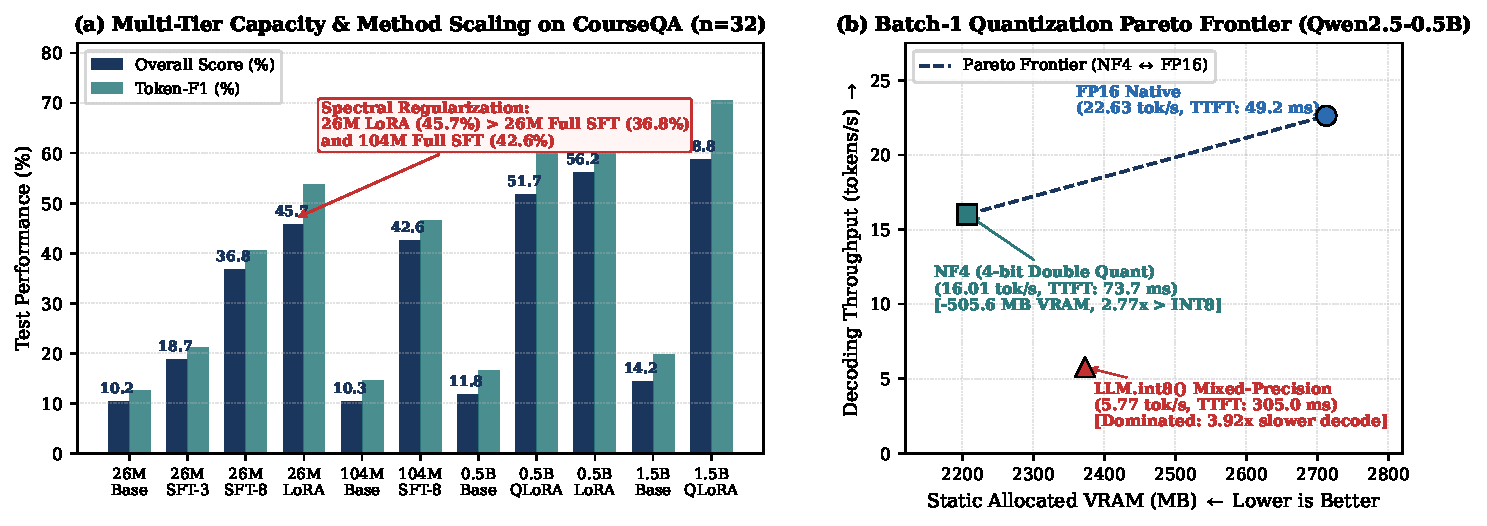
\includegraphics[width=\textwidth]{fig2_scaling_pareto.pdf}
  \caption{\textbf{Capacity scaling and quantization Pareto frontier.} \textbf{(a)} On \textsc{CourseQA}, rank-16 LoRA on \texttt{MiniMind-26M} ($45.71\%$) outperforms both 8-epoch Full SFT on \texttt{26M} ($36.80\%$) and 8-epoch Full SFT on \texttt{104M} ($42.56\%$), confirming low-rank spectral regularization (Proposition~\ref{prop:rank}). \textbf{(b)} Batch-1 quantization benchmark on \texttt{Qwen2.5-0.5B}: \texttt{NF4} and \texttt{FP16} form the latency--memory Pareto frontier, whereas \texttt{LLM.int8()} is strictly dominated due to outlier-decomposition synchronization overhead (Proposition~\ref{prop:quant}).}
  \label{fig:scaling_pareto}
\end{figure*}

\section{Main Results and Analysis}
\label{sec:results}

\subsection{Scaling Ladder and Spectral Regularization (Q1)}

Table~\ref{tab:main_results} and Figure~\ref{fig:scaling_pareto}(a) report performance across all four model tiers. Three findings stand out:

\paragraph{Low-rank adaptation beats Full SFT on compact domain corpora.}
On \texttt{MiniMind-26M} (\textsc{CourseQA}), increasing Full SFT from 3 epochs to 8 epochs raises \text{Overall} from $18.70\%$ to $36.80\%$ (EM $28.12\%$, Token-F1 $40.55\%$). Under the exact same 8-epoch budget, restricting updates to a rank-$16$ LoRA subspace achieves $45.71\%$ \text{Overall} (EM $40.62\%$, Token-F1 $53.70\%$, Contains $43.75\%$)---an $+8.91\%$ absolute improvement over 8-epoch Full SFT on the same $26\text{M}$ backbone, and $+3.15\%$ higher than 8-epoch Full SFT on the $4\times$ larger \texttt{MiniMind-104M} model ($42.56\%$). Simultaneously, LoRA reduces peak VRAM from $375.0\text{ MB}$ to $130.9\text{ MB}$ ($-65.1\%$). Consistent with Proposition~\ref{prop:rank}, rank truncation prevents small-sample memorization while preserving pre-trained representations.

\paragraph{Sub-billion SLMs achieve exact mastery on constrained syntax and out-of-template routing.}
Zero-shot baselines struggle with strict output constraints: \texttt{MiniMind-26M} scores $0.00\%$ schema validity on \textsc{JSONOut} ($3.91\%$ parse rate) and $0.00\%$ accuracy on \textsc{Intent} ($100.0\%$ unmapped conversational replies). \texttt{Qwen2.5-0.5B} parses valid JSON ($100.0\%$) but achieves only $57.03\%$ strict schema validity due to boolean type violations (emitting raw Chinese status tokens instead of JSON booleans), and scores $21.88\%$ on \textsc{Intent} ($38.54\%$ unmapped rate). After 4 epochs of assistant-masked fine-tuning, both \texttt{MiniMind-26M} (Full SFT) and \texttt{Qwen2.5-0.5B} (LoRA) reach $100.0\%$ JSON parse rate, $100.0\%$ strict schema validity, $100.0\%$ field accuracy, and $100.0\%$ out-of-template intent classification accuracy. Moreover, suppressing verbose zero-shot continuations reduces \texttt{MiniMind-26M} evaluation latency on \textsc{Intent} from $46.00\text{ s}$ to $11.80\text{ s}$ ($3.9\times$ speedup).

\paragraph{Monotonic capacity scaling on knowledge-intensive QA.}
On \textsc{CourseQA}, adapted performance scales monotonically with pre-trained capacity: from $45.71\%$ (\texttt{MiniMind-26M} LoRA) to $56.19\%$ (\texttt{Qwen2.5-0.5B} LoRA, EM $50.00\%$, Token-F1 $64.67\%$) and $58.80\%$ (\texttt{Qwen2.5-1.5B} QLoRA, EM $50.00\%$, Token-F1 $70.57\%$). Using 4-bit \texttt{NF4} double quantization (Eq.~\ref{eq:mem_qlora}), \texttt{Qwen2.5-1.5B} QLoRA training peaks at $4,715.1\text{ MB}$ VRAM ($31.6\%$ of T4 capacity), and on \texttt{Qwen2.5-0.5B}, QLoRA saves $261.0\text{ MB}$ peak training VRAM over \texttt{FP16} LoRA ($1,771.8\text{ MB}$ vs.\ $2,032.8\text{ MB}$) while retaining $92.0\%$ of its relative QA gain.

\begin{table}[t]
\centering
\resizebox{\columnwidth}{!}{%
\begin{tabular}{lrrrrrr}
\toprule
\textbf{Variant} & \textbf{Static MB} & \textbf{Peak MB} & \textbf{TTFT (ms)} & \textbf{Prefill/s} & \textbf{Decode/s} & \textbf{QA Score} \\
\midrule
\texttt{FP16} (Native) & 2712.7 & 2716.4 & \textbf{49.21} & \textbf{835.64} & \textbf{22.63} & 0.1178 \\
\texttt{LLM.int8()} & 2373.1 & 2378.8 & 305.02 & 190.33 & 5.77 & \textbf{0.1224} \\
\texttt{NF4} (4-bit DQ) & \textbf{2207.1} & \textbf{2217.3} & 73.65 & 578.19 & 16.01 & 0.1105 \\
\bottomrule
\end{tabular}%
}
\caption{\textbf{Batch-1 inference quantization benchmark on \texttt{Qwen2.5-0.5B}} (\textsc{CourseQA} test split, Tesla T4). \text{Static MB} and \text{Peak MB} denote allocated CUDA memory before and during generation.}
\label{tab:quant}
\end{table}

\subsection{Quantized Decoding Roofline and Pareto Frontier (Q3)}

Table~\ref{tab:quant} and Figure~\ref{fig:scaling_pareto}(b) compare native \texttt{FP16}, 8-bit mixed-precision decomposition (\texttt{LLM.int8()}; \citealp{dettmers2022llm}), and 4-bit NormalFloat with double quantization (\texttt{NF4}; \citealp{dettmers2023qlora}) on \texttt{Qwen2.5-0.5B}.

The measurements directly verify Proposition~\ref{prop:quant}. Although \texttt{LLM.int8()} reduces static memory by $339.6\text{ MB}$ ($2,712.7 \to 2,373.1\text{ MB}$) and preserves zero-shot QA accuracy ($0.1224$), it inflates TTFT by $6.20\times$ ($305.02\text{ ms}$ vs.\ $49.21\text{ ms}$) and reduces decoding throughput by $3.92\times$ ($5.77\text{ tok/s}$ vs.\ $22.63\text{ tok/s}$). Because \texttt{LLM.int8()} inspects activation magnitudes at every linear layer to route outlier channels ($|\mathbf{x}_j| > 6.0$) into \texttt{FP16} GEMMs before merging with \texttt{INT8} outputs, the per-token synchronization penalty ($t_{\text{dequant}} \approx 129.1\text{ ms/tok}$) overwhelms the $\sim 1.4\text{ ms/tok}$ GDDR6 bandwidth savings on a $494\text{M}$ model.

In contrast, 4-bit \texttt{NF4} relies on uniform blockwise lookup-table dequantization without dynamic activation branching. \texttt{NF4} achieves the lowest static memory footprint ($2,207.1\text{ MB}$, saving $505.6\text{ MB}$ over \texttt{FP16} and $166.0\text{ MB}$ over \texttt{INT8}) while sustaining $16.01\text{ tok/s}$ decoding throughput ($2.77\times$ faster than \texttt{LLM.int8()}) and $578.19\text{ tok/s}$ prefill speed ($3.04\times$ faster than \texttt{LLM.int8()}). Consequently, \texttt{FP16} and \texttt{NF4} define the deployment Pareto frontier on Turing GPUs.

\begin{figure*}[t]
  \centering
  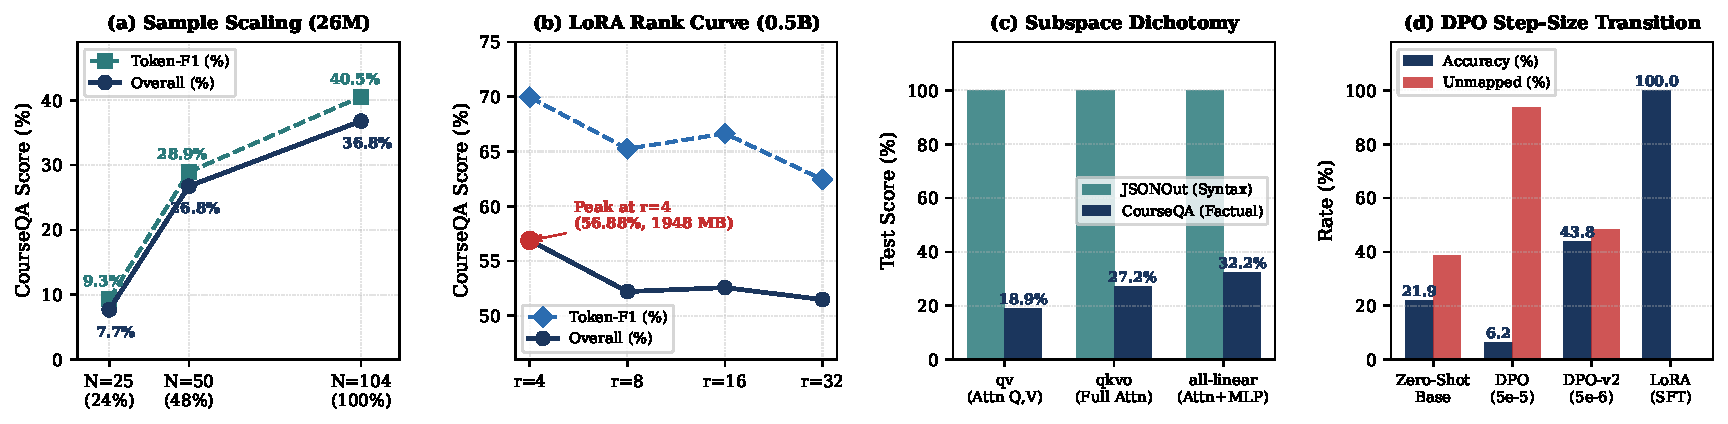
\includegraphics[width=\textwidth]{fig3_ablations_dpo.pdf}
  \caption{\textbf{Orthogonal ablations and preference alignment diagnostics.} \textbf{(a)} Sample-size scaling on \texttt{MiniMind-26M} (\textsc{CourseQA}, 8 ep Full SFT). \textbf{(b)} Inverted-U LoRA rank curve on \texttt{Qwen2.5-0.5B} (\textsc{CourseQA}, 6 ep), peaking at $r=4$ ($56.88\%$, Token-F1 $69.95\%$). \textbf{(c)} Subspace allocation dichotomy: \texttt{qv} saturates syntactic \textsc{JSONOut} ($100.0\%$), whereas factual \textsc{CourseQA} climbs monotonically from \texttt{qv} ($18.87\%$) to \texttt{qkvo} ($27.17\%$) and \texttt{all-linear} ($32.23\%$). \textbf{(d)} DPO learning-rate phase transition on \texttt{Qwen2.5-0.5B} (\textsc{Intent}), where $\eta = 5\times 10^{-6}$ recovers from likelihood displacement collapse.}
  \label{fig:ablations}
\end{figure*}

\begin{table}[t]
\centering
\resizebox{\columnwidth}{!}{%
\begin{tabular}{llrrrr}
\toprule
\textbf{Ablation Axis} & \textbf{Configuration} & \textbf{Metric 1} & \textbf{Metric 2} & \textbf{Overall} & \textbf{VRAM (MB)} \\
\midrule
\multicolumn{6}{l}{\textit{(A) Training Sample Size $N$ (\texttt{MiniMind-26M}, \textsc{CourseQA}, 8 ep Full SFT)}} \\
Sample Size & $N = 25$ (24\%) & EM: 0.0625 & F1: 0.0931 & 0.0767 & 375.0 \\
Sample Size & $N = 50$ (48\%) & EM: 0.2188 & F1: 0.2894 & 0.2675 & 376.9 \\
Sample Size & $N = 104$ (100\%) & \textbf{EM: 0.2812} & \textbf{F1: 0.4055} & \textbf{0.3680} & 375.0 \\
\midrule
\multicolumn{6}{l}{\textit{(B) Training Label Corruption $\eta_{\text{noise}}$ (\texttt{MiniMind-26M}, \textsc{Intent}, 4 ep Full SFT)}} \\
Label Noise & $\eta_{\text{noise}} = 0\%$ & \textbf{Acc: 1.0000} & \textbf{F1: 1.0000} & \textbf{1.0000} & 376.8 \\
Label Noise & $\eta_{\text{noise}} = 20\%$ & Acc: 0.9792 & F1: 0.9783 & 0.9792 & 375.6 \\
Label Noise & $\eta_{\text{noise}} = 50\%$ & Acc: 0.5677 & F1: 0.4743 & 0.5677 & 376.0 \\
\midrule
\multicolumn{6}{l}{\textit{(C) LoRA Rank $r$ (\texttt{Qwen2.5-0.5B}, \textsc{CourseQA}, 6 ep, $\alpha = 2r$, \texttt{all-linear})}} \\
Adapter Rank & $r = 4, \alpha = 8$ & \textbf{EM: 0.5000} & \textbf{F1: 0.6995} & \textbf{0.5688} & \textbf{1948.1} \\
Adapter Rank & $r = 8, \alpha = 16$ & EM: 0.4688 & F1: 0.6525 & 0.5221 & 1972.0 \\
Adapter Rank & $r = 16, \alpha = 32$ & EM: 0.4688 & F1: 0.6664 & 0.5257 & 2022.6 \\
Adapter Rank & $r = 32, \alpha = 64$ & EM: 0.4375 & F1: 0.6243 & 0.5148 & 2122.9 \\
\bottomrule
\end{tabular}%
}
\caption{\textbf{Orthogonal ablations on sample size (A), label corruption (B), and LoRA rank (C).} All runs fix random seed $42$.}
\label{tab:ablations_abc}
\end{table}

\subsection{Orthogonal Ablations and Subspace Allocation (Q1, Q2)}
\label{sec:exp_ablation}

Tables~\ref{tab:ablations_abc} and~\ref{tab:ablation_target} and Figure~\ref{fig:ablations}(a--c) report four orthogonal ablations holding all non-ablated hyperparameters constant:

\paragraph{Sample scaling and label-noise phase transition.}
In Table~\ref{tab:ablations_abc}(A), $N=25$ examples ($\sim 3$ per topic) fail to reach the critical sample threshold on \textsc{CourseQA} ($0.0767$ \text{Overall}); doubling to $N=50$ yields a $3.49\times$ jump to $0.2675$, and $N=104$ reaches $0.3680$. In Table~\ref{tab:ablations_abc}(B), \texttt{MiniMind-26M} exhibits strong resilience to moderate label corruption on \textsc{Intent}: at $\eta_{\text{noise}} = 20\%$, test accuracy remains $97.92\%$ (Macro-F1 $97.83\%$), as coherent clean-label gradients dominate early optimization \citep{arpit2017closer}. At $\eta_{\text{noise}} = 50\%$, accuracy drops to $56.77\%$ (Macro-F1 $47.43\%$), yet the unmapped rate remains $0.00\%$---indicating that output vocabulary syntax is preserved even under severe semantic label noise.

\paragraph{The inverted-U LoRA rank curve.}
Sweeping $r \in \{4, 8, 16, 32\}$ with $\alpha = 2r$ on \texttt{Qwen2.5-0.5B} (\textsc{CourseQA}, Table~\ref{tab:ablations_abc}C, Figure~\ref{fig:ablations}b) reveals a non-monotonic curve peaking at $r=4$ (\text{Overall} $56.88\%$, EM $50.00\%$, Token-F1 $69.95\%$, Contains $53.12\%$) with the lowest memory footprint ($1,948.1\text{ MB}$). Increasing rank to $r=32$ lowers \text{Overall} by $-5.40\%$ to $51.48\%$ (Token-F1 $62.43\%$) while consuming $+174.8\text{ MB}$ additional VRAM. This confirms Proposition~\ref{prop:rank}: on compact domain datasets, minimal rank $r=4$ captures the task subspace while higher ranks reintroduce overfitting.

\begin{table}[t]
\centering
\resizebox{\columnwidth}{!}{%
\begin{tabular}{llrrrr}
\toprule
\textbf{Task Regime} & \textbf{Target Subspace} & \textbf{Metric 1} & \textbf{Metric 2} & \textbf{Overall} & \textbf{VRAM (MB)} \\
\midrule
\multicolumn{6}{l}{\textit{Syntax-Constrained Regime: \textsc{JSONOut} (4 ep, $r=16$, $\text{grad\_accum}=4$)}} \\
\textsc{JSONOut} & \texttt{qv} ($W_q, W_v$) & Parse: 1.0000 & Field: 1.0000 & \textbf{1.0000} & \textbf{1935.9} \\
\textsc{JSONOut} & \texttt{qkvo} ($\mathcal{M}_{\text{attn}}$) & Parse: 1.0000 & Field: 1.0000 & \textbf{1.0000} & 1948.3 \\
\textsc{JSONOut} & \texttt{all-linear} ($\mathcal{M}_{\text{all}}$) & Parse: 1.0000 & Field: 1.0000 & \textbf{1.0000} & 2024.3 \\
\midrule
\multicolumn{6}{l}{\textit{Knowledge-Intensive Regime: \textsc{CourseQA} (3 ep, $r=16$, $\text{grad\_accum}=2$)}} \\
\textsc{CourseQA} & \texttt{qv} ($W_q, W_v$) & EM: 0.0000 & F1: 0.2767 & 0.1887 & \textbf{1933.3} \\
\textsc{CourseQA} & \texttt{qkvo} ($\mathcal{M}_{\text{attn}}$) & EM: 0.0625 & F1: 0.3853 & 0.2717 & 1945.4 \\
\textsc{CourseQA} & \texttt{all-linear} ($\mathcal{M}_{\text{all}}$) & \textbf{EM: 0.1250} & \textbf{F1: 0.4343} & \textbf{0.3223} & 2021.3 \\
\bottomrule
\end{tabular}%
}
\caption{\textbf{Target subspace ablation on \texttt{Qwen2.5-0.5B}} contrasting attention-only (\texttt{qv}, \texttt{qkvo}) against full linear (\texttt{all-linear}: attention + SwiGLU MLP) adapters across syntactic (\textsc{JSONOut}) and factual (\textsc{CourseQA}) regimes.}
\label{tab:ablation_target}
\end{table}

\paragraph{Subspace dichotomy between syntactic routing and factual memory.}
Table~\ref{tab:ablation_target} and Figure~\ref{fig:ablations}(c) test Inequality~(\ref{eq:subspace_ineq}) directly on \texttt{Qwen2.5-0.5B}. On \textsc{JSONOut}, adapting $\mathcal{M}_{\text{qv}} = \{W_q, W_v\}$ alone achieves $100.0\%$ schema validity and $100.0\%$ field accuracy; expanding to \texttt{qkvo} or \texttt{all-linear} provides zero accuracy lift while adding $88.4\text{ MB}$ of VRAM overhead. On \textsc{CourseQA} (evaluated at 3 epochs, $\text{grad\_accum}=2$ to isolate early subspace learning speed), \texttt{qv}-only adaptation reaches only $18.87\%$ \text{Overall} (EM $0.00\%$, Token-F1 $27.67\%$, Contains $3.12\%$). Unlocking full attention (\texttt{qkvo}) lifts \text{Overall} by $+8.30\%$ to $27.17\%$ (EM $6.25\%$, Token-F1 $38.53\%$), and unlocking the SwiGLU FFN projections (\texttt{all-linear}: \texttt{gate\_proj}, \texttt{up\_proj}, \texttt{down\_proj}) adds a further $+5.06\%$ to reach $32.23\%$ (EM $12.50\%$, Token-F1 $43.43\%$, a $+13.36\%$ total gain over \texttt{qv}). This confirms that factual adaptation requires modifying FFN key-value memories \citep{geva2021transformer}, whereas syntactic formatting only requires attention re-routing.

\begin{table}[t]
\centering
\resizebox{\columnwidth}{!}{%
\begin{tabular}{llrrrr}
\toprule
\textbf{Alignment Regime} & \textbf{Hyperparameters} & \textbf{Acc} & \textbf{Macro-F1} & \textbf{Unmapped} & \textbf{VRAM (MB)} \\
\midrule
Zero-Shot Baseline & --- & 0.2188 & 0.1903 & 0.3854 & 2024.8 \\
DPO (High Step) & $\beta=0.1, \eta=5\times 10^{-5}$ & 0.0625 & 0.0889 & 0.9375 & 2025.4 \\
\textbf{DPO (Bounded Step)} & $\beta=0.1, \eta=5\times 10^{-6}$ & \textbf{0.4375} & \textbf{0.4759} & 0.4844 & \textbf{971.2} \\
Supervised LoRA & $r=16, \eta=3\times 10^{-4}$ & \textbf{1.0000} & \textbf{1.0000} & \textbf{0.0000} & 2025.4 \\
\bottomrule
\end{tabular}%
}
\caption{\textbf{Preference alignment stability on \texttt{Qwen2.5-0.5B}} (\textsc{Intent}, $n=192$ test queries) across DPO step sizes vs.\ Zero-Shot and Supervised LoRA.}
\label{tab:dpo}
\end{table}

\subsection{Preference Alignment: DPO Step-Size Phase Transition (Q4)}

Table~\ref{tab:dpo} and Figure~\ref{fig:ablations}(d) evaluate DPO on \texttt{Qwen2.5-0.5B} (\textsc{Intent}), where each training prompt $x$ pairs its ground-truth label $y_w$ against a corrupted negative label $y_l$.

At $\eta = 5\times 10^{-5}$, DPO exhibits severe likelihood displacement (Section~\ref{sec:dpo_theory}): accuracy drops from $21.88\%$ (Zero-Shot) to $6.25\%$, while the unmapped rate spikes to $93.75\%$ as the policy emits off-manifold English phrases (e.g., ``good weather!'') that share zero tokens with the penalized snake\_case labels. Lowering the step size by one order of magnitude to $\eta = 5\times 10^{-6}$ (\texttt{dpo-v2}) stabilizes the reference KL constraint, lifting accuracy by $7.0\times$ to $43.75\%$ and Macro-F1 to $47.59\%$ ($2.0\times$ above Zero-Shot). Even in the stable regime, however, standalone DPO trails supervised LoRA ($100.0\%$), because pairwise repulsion against a single negative label $y_l$ per query does not suppress the remaining four incorrect classes.

\paragraph{Claim boundary.}
Propositions~\ref{prop:quant} and~\ref{prop:rank} characterize hardware latency bounds and linear update rank ceilings; they do not claim universal numerical values for $r^*$ across arbitrary pre-training corpora. Empirically, our $100.0\%$ results on \textsc{JSONOut} and \textsc{Intent} establish that $26\text{M}$--$0.5\text{B}$ SLMs can master strict 4-schema extraction and 6-way out-of-template classification; they do not imply that $26\text{M}$ models match frontier LLMs on open-ended reasoning, where capacity bounds remain binding (\textsc{CourseQA} $45.71\%$ at $26\text{M}$ vs.\ $58.80\%$ at $1.5\text{B}$).

\section{Related Work}

\paragraph{Parameter-efficient adaptation and intrinsic dimensionality.}
\citet{aghajanyan2021intrinsic} showed that pre-trained language models possess a low intrinsic dimension during fine-tuning, motivating LoRA \citep{hu2022lora}, adaptive rank allocation \citep{zhang2023adalora}, and quantized backpropagation via QLoRA \citep{dettmers2023qlora}. While prior work primarily treats LoRA as a memory-reduction approximation for $7\text{B}$+ models, we show that in sub-billion SLMs ($26\text{M}$--$0.5\text{B}$) trained on compact domain datasets, rank truncation ($r \in [4, 16]$) acts as a spectral regularizer that substantially outperforms full-parameter SFT.

\paragraph{Mechanistic localization and edge quantization.}
\citet{geva2021transformer} and \citet{meng2022locating} demonstrated that Transformer MLP layers operate as key-value memories encoding factual knowledge. Our target-subspace ablation connects this mechanistic finding to PEFT design, explaining why \texttt{qv} adapters saturate syntactic extraction while MLP adapters are required for domain QA. On the deployment side, \texttt{LLM.int8()} \citep{dettmers2022llm} and \texttt{NF4} \citep{dettmers2023qlora} compress model weights, but our Roofline analysis \citep{williams2009roofline} and Turing \texttt{sm\_75} benchmarks reveal that dequantization kernel latency governs batch-1 decoding throughput.

\paragraph{Direct preference optimization.}
\citet{rafailov2023direct} formulated DPO as a closed-form alternative to RLHF. Subsequent studies identified likelihood displacement under offline preference training \citep{pal2024smaug,tajwar2024preference}; our results isolate the step-size phase transition governing this failure mode on discrete classification manifolds.

\section{Limitations}
\label{sec:limitations}

\paragraph{Hardware scope and batching regime.}
Our Roofline latency measurements are conducted on an NVIDIA Turing \texttt{sm\_75} GPU at batch size $B=1$ to reflect single-user edge deployment. On newer Hopper/Blackwell architectures with native \texttt{FP8}/\texttt{INT4} tensor instructions or under large-batch continuous batching ($B \ge 32$) where decoding becomes compute-bound ($\mathcal{I}_{\text{decode}} > \mathcal{I}^*$), the relative throughput ratio between \texttt{INT8} and \texttt{FP16} will shift.

\paragraph{Capacity ceiling on multi-hop reasoning.}
Qualitative error inspection on \textsc{CourseQA} shows that while \texttt{MiniMind-26M} LoRA masters single-concept definitions, it still confuses closely related multi-hop concepts (e.g., conflating Prim's and Kruskal's greedy strategies on minimum spanning trees), whereas \texttt{Qwen2.5-1.5B} QLoRA resolves them. Low-rank adaptation optimizes extraction of pre-trained representations but cannot substitute for base-model capacity when pre-training exposure is absent.

\section{Conclusion}

We formulated and empirically validated a first-principles framework for adapting and quantizing Small Language Models ($26\text{M}$--$1.5\text{B}$) under edge hardware constraints. Across 39 controlled runs, we showed that (i) low-rank adaptation ($r \in [4, 16]$) acts as a spectral regularizer that outperforms Full SFT by $+8.91\%$ on compact domain QA; (ii) attention-only (\texttt{qv}) adapters saturate syntactic JSON extraction ($100.0\%$), whereas domain QA requires unlocking FFN projections ($+13.36\%$ gain); (iii) 4-bit \texttt{NF4} dominates \texttt{LLM.int8()} by $2.77\times$ in batch-1 decoding throughput while saving $505.6\text{ MB}$ of static VRAM; and (iv) bounding DPO step sizes to $\eta \le 5\times 10^{-6}$ prevents likelihood displacement on compact classification manifolds.

\bibliographystyle{plainnat}
\bibliography{references}

\end{document}
